%%%%%%%%%%%%%%%%%%%%%%%%%%%%%%%%%%%%%%%%%%%%%%%%%%%%%%
% LaTeX Template for UMD Assignments.
% Created by Jason Filippou (jasonfil@cs.umd.edu)
% Maintained at: https://github.com/JasonFil/UMDAssignmentTemplates
% Check LICENSE file on GitHub for licensing. 

% Look for the string "STUDENT" to find comments about where you can answer the problems
% if you choose to do LaTeX.
%%%%%%%%%%%%%%%%%%%%%%%%%%%%%%%%%%%%%%%%%%%%%%%%%%%%%%

% Document class will always be article for the purposes of UMD assignments
\documentclass[letterpaper,12pt]{article}


%%%%%%%%%%%%%  IMPORT MACRO FILES AS NEEDED %%%%%%%%%%%
\usepackage{amsgen,amsmath,amstext,amsbsy,amsopn,amssymb,amsthm}
\usepackage[usenames,dvipsnames,svgnames,table]{xcolor}
\usepackage{array, nicefrac, mathtools}
\usepackage[bottom]{footmisc} % To keep the footnote at the bottom even after putting answering environments.
\usepackage{verbatim}
\usepackage{booktabs} % for multicolumn
\usepackage[font=normalsize,skip=0pt, justification=centering]{caption, subcaption}
\usepackage[colorlinks=true,linkcolor=blue,urlcolor=blue]{hyperref}
\usepackage{float,relsize,setspace,enumitem,pbox,cleveref,multicol}
\usepackage{censor}
\usepackage{textcomp} % for the cent symbol
\usepackage{multido}
\usepackage{bbding} % Has a checkmark symbol reachable through \Checkmark
\usepackage{tikz}
% Basic math
%\usepackage{amsgen,amsmath,amstext,amsbsy,amsopn,amssymb,amsthm}
%\usepackage[usenames,dvipsnames,svgnames,table]{xcolor}
%\usepackage{array, nicefrac, mathtools}

% Theorems, definitions, equations, lemmas
\newtheorem{thm}{Theorem}[section]
\newtheorem{prop}[thm]{Proposition}
\newtheorem{lem}[thm]{Lemma}
\newtheorem{cor}[thm]{Corollary}
\newtheorem{defn}{Definition}
\newtheorem{rem}[thm]{Remark}
\numberwithin{equation}{section}
\newtheorem*{defn*}{Definition} % Theorem environments with no numbering
\newtheorem*{prop*}{Proposition}
\newtheorem*{thm*}{Theorem}

% For negation and quantifiers in Discrete Math
\newcommand{\shortsim}{\raise.17ex\hbox{$\scriptstyle \sim$}}
\renewcommand{\neg}{\shortsim}
\renewcommand{\nexists}{\neg\exists}
\newcommand{\nequiv}{\ensuremath{\not\equiv}}

% Some larger symbols for clarity.
\newcommand{\Sum}{\ensuremath{\mathlarger{\sum}}}
\newcommand{\Prod}{\ensuremath{\mathlarger{\prod}}}
\newcommand{\Ell}{\ensuremath{\mathcal{L}}}
\DeclarePairedDelimiter{\ceil}{\lceil}{\rceil}
\DeclarePairedDelimiter{\floor}{\lfloor}{\rfloor}

%Some number sets
\newcommand{\N}{\ensuremath{\mathbb{N}}}
\newcommand{\Nplus}{\ensuremath{\mathbb{N}^+}}
\newcommand{\Nstar}{\ensuremath{\mathbb{N}^*}} % pretty much equivalent to Nplus
\newcommand{\Neven}{\ensuremath{\mathbb{N}^\text{even}}}
\newcommand{\Nstareven}{\ensuremath{\mathbb{N}^*_\text{even}}}
\newcommand{\Nodd}{\ensuremath{\mathbb{N}^\text{odd}}}
\newcommand{\Z}{\ensuremath{\mathbb{Z}}}
\newcommand{\Zstar}{\ensuremath{\mathbb{Z}^*}}
\newcommand{\Zstareven}{\ensuremath{\mathbb{Z}^*_\text{even}}}
\newcommand{\Zplus}{\ensuremath{\mathbb{Z}^+}}
\newcommand{\Zminus}{\ensuremath{\mathbb{Z}^-}}
\newcommand{\Zeven}{\ensuremath{\mathbb{Z}^\text{even}}}
\newcommand{\Zodd}{\ensuremath{\mathbb{Z}^\text{odd}}}
\newcommand{\Q}{\ensuremath{\mathbb{Q}}}
\newcommand{\Qplus}{\ensuremath{\mathbb{Q}^+}}
\newcommand{\Qstar}{\ensuremath{\mathbb{Q}^*}}
\newcommand{\Qminus}{\ensuremath{\mathbb{Q}^-}}
\newcommand{\R}{\ensuremath{\mathbb{R}}}
\newcommand{\Rminus}{\ensuremath{\mathbb{R}^-}}
\newcommand{\Rplus}{\ensuremath{\mathbb{R}^+}}
\newcommand{\Rstar}{\ensuremath{\mathbb{R}^*}}
\newcommand{\I}{\ensuremath{\mathbb{R - Q}}}
\renewcommand{\P}{\ensuremath{\mathbf{P}}}
\newcommand{\Pset}[1]{\ensuremath{\mathcal{P}(#1)}}

% An explained mathematical derivation in the form of an unbulleted list item.
\newcommand{\derivitem}[2]{\item[] $=#1 \qquad \qquad $ \derivexpl{#2}}
\newcommand{\derivitemnte}[2]{\item[] $#1 \qquad \qquad $ \derivexpl{#2}}
\newcommand{\derivitemized}[2]{\item $=#1 \qquad \qquad $ \derivexpl{#2}}
\newcommand{\derivitemizednte}[2]{\item $#1 \qquad \qquad $ \derivexpl{#2}}

% Math and lines.
\newcommand{\mathitem}[1]{\item $#1$ \hrulefill}

% Induction-related
\newcommand{\indstart}[1]{Let $P($#1$)$ be the proposition we are attempting to prove true. We proceed via mathematical induction on #1.}
\newcommand{\IB}{\textbf{Inductive Base: }}
\newcommand{\IH}{\textbf{Inductive Hypothesis: }}
\newcommand{\IS}{\textbf{Inductive Step: }}
\newcommand{\derivexpl}[1]{\text{ \emph { (#1) } } \\ } % Textual explanation of line-by-line derivations

% Interesting mathematical notation and symbols

\newcommand{\bigoh}[1]{$\mathcal O$(#1)}
\newcommand{\bigtheta}[1]{$\mathit{\Theta}$(#1)}
\newcommand{\bigomega}[1]{$\mathit{\Omega}$(#1)}

% For logical rules of inference

\newcommand{\rulesofinference}[2]{
	\begin{table}[H]
		\centering
		\begin{tabular}{|c|c|p{2.5cm}|p{2.5cm}|}\hline
			\centering
			\textbf{Modus Ponens} & \textbf{Modus Tollens} & \textbf{Disjunctive addition} & \textbf{Conjunctive addition} \\ \hline
				$\begin{aligned}
			p  \\
			p \Rightarrow q \\
			\therefore q
		\end{aligned}$ & 
		 $\begin{aligned}
			\neg q  \\
			p \Rightarrow q \\
			\therefore \neg p
		\end{aligned}$ & 
		 $\begin{aligned}
			p  \\
			\therefore p \lor q
		\end{aligned}$ &
		$\begin{aligned}
			p, q \\
			\therefore p \land q
		\end{aligned}$ \\ \hline 
			 \textbf{Conjunctive Simplification} & \textbf{Disjunctive syllogism} & \textbf{Hypothetical syllogism} &  \textbf{Resolution}  \\ \hline
			 $\begin{aligned}
			p \land q \\
			\therefore p, q
		\end{aligned}$ 	& 
			$\begin{aligned}
			p \lor q \\
			\neg p \\
			\therefore q
		\end{aligned}$ &
		$\begin{aligned}
			p  \Rightarrow q \\
			q \Rightarrow r \\
			\therefore p \Rightarrow r
		\end{aligned}$ &  
		$\begin{aligned}
		p \lor q\\
		(\neg q) \lor z\\
		\therefore p \lor z
		\end{aligned}$ \\ \hline
		\end{tabular}
		\caption{#1}
		\label{#2}
	\end{table}
}

\newcommand{\logicalequivs}[2]{

	\begin{table}[H]
		\centering
		\renewcommand*{\arraystretch}{1.2}
		\begin{tabular}{|>{\centering\arraybackslash}p{2.5in} | c | c |} \hline
			\textbf{Commutativity of binary operators} & $p \land q \equiv q \land p$ & $p \lor q \equiv q \lor p$ \\ \hline
		\textbf{Associativity of binary operators} & $(p \land q) \land r \equiv p \land (q \land r)$ &  $(p \lor q) \lor r \equiv p \lor (q \lor r)$ \\ \hline
		\textbf{Distributivity of binary operators} & $p \land (q \lor r) \equiv (p \land q) \lor (p \land r)$ & $p \lor (q \land r) \equiv (p \lor q) \land (p \lor r)$ \\ \hline
		\textbf{Identity laws} & $p \land T \equiv p$ & $p \lor F \equiv p$ \\ \hline
		\textbf{Negation laws} & $p \lor (\neg p) \equiv T$ & $p \land (\neg p) \equiv F$ \\ \hline
		\textbf{Double negation} & \multicolumn{2}{c|}{$\neg (\neg p) \equiv p$}  \\ \hline 
		\textbf{Idempotence} & $p \land p \equiv p$ & $p \lor p \equiv p$ \\ \hline
		\textbf{De Morgan's axioms} & $\neg (p \land q) \equiv (\neg p )\lor (\neg q)$ & $\neg (p \lor q) \equiv (\neg p) \land (\neg q)$\\ \hline
		\textbf{Universal bound laws} & $p \lor T \equiv T$ & $p \land F \equiv F$ \\ \hline
		\textbf{Absorption laws} & $p \lor (p \land q) \equiv p$ & $p \land (p \lor q) \equiv p$ \\ \hline
		\textbf{Negations of contradictions / tautologies} & $\neg F \equiv T$ & $\neg T \equiv F$ \\ \hline
		\textbf{Contrapositive} & \multicolumn{2}{c|}{$(a \Rightarrow b) \equiv (( \neg b) \Rightarrow (\neg a))$} \\ \hline
		\textbf{Equivalence between biconditional and implication} & \multicolumn{2}{c|}{$a \Leftrightarrow b \equiv (a \Rightarrow b) \land (b \Rightarrow a)$} \\ \hline
		\textbf{Equivalence between implication and disjunction} & \multicolumn{2}{c|}{$a \Rightarrow b \equiv \neg a \lor b$} \\ \hline
		\end{tabular} \vspace{.1in}
		\caption{#1}
		\label{#2}
	\end{table}
}

\newcommand{\settheory}[2]{
	\begin{table}[H]
		\centering
		\renewcommand*{\arraystretch}{1.4}
		\begin{tabular}{| c | c | c | } \hline 
			{\large \bf Operation} & 		{\large \bf Symbol} &  {\large \bf Definition } \\  \hline 
			\textbf{Membership} & $x \in A$ & $x$ is a member of set $A$ \\ \hline
			\textbf{Non-membership} & $x \notin A$ & $ \neg (x \in A)$ \\ \hline
			\textbf{Union} & $A \cup B$ & $\{ (x \in A) \lor (x \in B)$\}   \\ \hline
			\textbf{Intersection} & $A \cap B$ & $\{ (x \in A) \land (x \in B)$\}   \\ \hline
			\textbf{Relative complement of} $\mathbf B$ \textbf{given} $\mathbf A$ & $A - B$ & $\{ (x \in A) \land (x \notin B)$\}   \\ \hline 
			\textbf{Universal (Absolute) complement} & $A^c$ & $\{x \notin A\}$\\ \hline
			\textbf{Cartesian Product} & $A \times B$ & $\{(a, b) \mid   (a \in A) \land (b \in B)  \}$ \\ \hline
			\textbf{Subset} & $A \subseteq B$ & $(\forall x \in A)[x \in B] $\\ \hline
			\textbf{Superset} & $A \supseteq B$ & $ B \subseteq A$\\ \hline
			\textbf{Set equality} & $A = B$ & $(A \subseteq B) \land (B \subseteq A) $ \\ \hline
			\textbf{Set non-equality} & $A \neq  B$ & $\neg (A =B) $ \\ \hline
			\textbf{Proper subset} & $A \subset B$ & $ \{ (A \subseteq B) \land (A \neq B) \} $ \\ \hline
			\textbf{Proper superset} & $A \supset B$ & $ \{ (A \supseteq B) \land (A \neq B) \} $ \\ \hline
			\textbf{Powerset} & $\Pset{A} $ & $ \{ X \mid X \subseteq A \} $ \\ \hline
		\end{tabular}
		\vspace{.1in}
		\caption{#1}
		\label{#2}
	\end{table}
}

% A useful environment for the questions where I ask students to provide two infinite domains
% which make a quantified statement true and false. Needs \myline.

\newcommand{\innerlist}{
	\begin{itemize}
		\setlength\itemsep{1em}	
		\item[-] $D_T=$ \myline{2in}
		\item[-] $D_F=$ \myline{2in}
	\end{itemize}
}

% Induction - related
\newcommand{\indbase}[1]{
	\begin{center}
		\textbf{WRITE YOUR INDUCTIVE BASE BELOW THIS LINE} \\
		\hrulefill
	\end{center}
   	\vspace{#1}
}

\newcommand{\indhypothesis}[1]{
	\begin{center}
		\textbf{WRITE YOUR INDUCTIVE HYPOTHESIS BELOW THIS LINE} \\
		\hrulefill
	\end{center}
   	\vspace{#1}
}


\newcommand{\indstep}[1]{
	\begin{center}
		\textbf{WRITE YOUR INDUCTIVE STEP BELOW THIS LINE} \\
		\hrulefill
	\end{center}
   	\vspace{#1}
}


\newcommand{\contindbase}[1]{
	\begin{center}
		\textbf{CONTINUE YOUR INDUCTIVE BASE BELOW THIS LINE} \\
		\hrulefill
	\end{center}
   	\vspace{#1}
}

\newcommand{\contindhypothesis}[1]{
	\begin{center}
		\textbf{CONTINUE YOUR INDUCTIVE HYPOTHESIS BELOW THIS LINE} \\
		\hrulefill
	\end{center}
   	\vspace{#1}
}


\newcommand{\contindstep}[1]{
	\begin{center}
		\textbf{CONTINUE YOUR INDUCTIVE STEP BELOW THIS LINE} \\
		\hrulefill
	\end{center}
   	\vspace{#1}
}


\newcommand{\standardinductionspace}{
	\indbase{2.5in}
	\indhypothesis{1.5in}
	\pagebreak
	\indstep{\paperheight}
} % Lots of math symbols 
% Source code, mainly for Data Structures
\definecolor{DarkGray}{gray}{0.35}
\definecolor{dkgreen}{rgb}{0, 1, 0}
\definecolor{mauve}{rgb}{78, 9,117}
\usepackage{listings, textcomp, upquote}
\lstset{
  language=Java,
  upquote=true;
  aboveskip=3mm,
  belowskip=3mm,
  showstringspaces=false,
  columns=flexible,
  numbers=left,
  basicstyle={\small\ttfamily},
  numberstyle=\tiny\color{black},
  keywordstyle=\color{blue},
  commentstyle=\color{DarkGray},
  stringstyle=\color{ForestGreen},
  breaklines=true,
  breakatwhitespace=true,
  tabsize=3
} % This is useful for assignments in CMSC420, 132, etc
\newcommand{\myline}[1]{\underline{\hspace{#1}}}
\newcounter{problems}
\newcounter{questions}[problems]
\newcounter{subquestions}[questions]
\newcommand{\problem}[2]{\stepcounter{problems} {\Large \bf \noindent Problem \arabic{problems}: #1 \emph{(#2 pts)}} \\[.4cm]}
\newcommand{\question}[2]{\stepcounter{questions} \noindent{\emph{\Large Question (\alph{questions}): #1 (#2 pts) }\\[.4cm]}}
\newcommand{\subquestion}[2]{\stepcounter{subquestions} \noindent{\emph{\Large Subquestion (\roman{subquestions}): #1 (#2 pts) }\\[.4cm]}}

% Some standard centering and italicization of text.
\newcommand{\frontrowcenter}[1]{\begin{center}{\em \Large  #1  }\end{center}}

% A blank page
\newcommand{\blankpage}{
\clearpage
\vspace*{\fill}
	\begin{minipage}{\textwidth}
		\hspace{.5in} \Large \textbf{THIS PAGE INTENTIONALLY LEFT BLANK}\\
	\end{minipage}
\vfill % equivalent to \vspace{\fill}
\clearpage
}

\newcommand{\answerspace}[1]{
	\begin{center}
		\textbf{BEGIN YOUR ANSWER BELOW THIS LINE} \\ \hrulefill \vspace{#1} \\ \hrulefill
	\end{center}
}

\newcommand{\answerspacefullpage}{
	\begin{center}
		\textbf{BEGIN YOUR ANSWER BELOW THIS LINE} \\ \hrulefill \pagebreak
	\end{center}
}


\newcommand{\additionalanswerspace}[1]{
	\begin{center}
		\textbf{CONTINUE YOUR ANSWER FOR #1 BELOW THIS LINE } \\ \hrulefill \vspace{#1} \\ \hrulefill
	\end{center}
}

\newcommand{\additionalanswerspacefullpage}{
	\begin{center}
		\textbf{CONTINUE YOUR ANSWER BELOW THIS LINE} \\ \hrulefill \pagebreak
	\end{center}
}

\newcommand{\freespace}[1]{
	\begin{center}
		\large \textbf{SCRAP SPACE BELOW} \\ 
		\hrulefill
		\pagebreak 
	\end{center}
}

\newcommand{\silentanswerspace}[1]{
	\\ \hrule \vspace{#1} \hrule 
}


\newcommand{\notespage}{
	\pagebreak
	\begin{center}
		\Large \textbf{SCRAP PAPER} \\ \hrulefill
	\end{center}
	\pagebreak
}

\newcommand{\showyourwork}{
	\begin{center}
		\large \textbf{SHOW YOUR WORK BELOW} \\ 
		\hrulefill
		\pagebreak
	\end{center}
}

\newcommand{\justifywork}{
	\begin{center}
		\large \textbf{JUSTIFY YOUR ANSWERS BELOW} \\ 
		\hrulefill
		\pagebreak
	\end{center}
}

% Space for T/F:
\newcommand{\tfline}{\myline{.5cm}}

% For sets:
\newcommand{\curlybraces}[1]{\ensuremath{\lbrace #1 \rbrace}}

% For cardinalities:
\newcommand{\crd}[1]{\ensuremath{ \big \vert #1 \big \vert }}

\newcommand{\yesno}{{\footnotesize YES / NO}}
\newcommand{\truefalse}{{\normalsize  \bf TRUE / FALSE}}

% \item environments coupled with a line at the end, for students to write T and F in.
\newcommand{\tfitem}[1]{\item #1 \null\hfill \framebox(25,25){} \\ \hdashrule{0.95\textwidth}{1pt}{2pt}}
\newcommand{\setitem}[1]{\tfitem{$\curlybraces{#1}$} }
\newcommand{\lineitem}[2]{\item #1 \null \hfill \myline{#2}}

% Some circles and squares for students to fill in.
\newcommand{\whitecircle}[1]{\tikz[baseline=-0.5ex]\draw[black, radius=#1] (0,0) circle ;}
\newcommand{\whitesquare}[1]{\tikz[baseline=-0.5ex]\draw[black] (0,0) rectangle(#1, #1) ;}
% Emphasis
\newcommand{\F}{$\mathbf{F}$}
\newcommand{\T}{$\mathbf{T}$}
\newcommand{\False}{\textbf{False}}
\newcommand{\false}{\textbf{false}}
\newcommand{\True}{\textbf{True}}
\newcommand{\true}{\textbf{true}}
\newcommand{\TODO}{\textcolor{red}{\textbf{TODO}}}
\newcommand{\TBD}{\textcolor{red}{\textbf{TBD}}}
\newcommand{\codeemph}[1]{\texttt{\textbf{#1}}}
\newcommand{\Red}{\textcolor{red}{Red}}
\newcommand{\red}{\textcolor{red}{red}}
\newcommand{\makered}[1]{\textcolor{red}{#1}}
\newcommand{\Rbbst}{\textcolor{red}{Red}-black tree}
\newcommand{\rbbst}{\textcolor{red}{red}-black tree}
\newcommand{\nullc}{\texttt{\textbackslash 0}}
\newcommand{\SPC}{\texttt{SPC}}
\newcommand{\checkmarkifsoln}{\ifshowsoln \textcolor{red}{\Checkmark} \fi}
\newcommand{\dialitem}[2]{\item[-] \textbf{#1}: ``\textit{#2}"} % For dialogue building.
% Repeating commands many times!
\newcommand{\Repeat}{\multido{\i=1+1}} 

\newcommand{\homeworkdata}[3]{

		\noindent\makebox[\textwidth]{\LARGE \bf #1, #2 }
		\ \\
		\noindent\makebox[\textwidth]{\Large \bf  Homework \##3 }
	
		\ \\
		% STUDENT: If you want to change your first and last name, all you have to do is replace \myline{4in} with \underline{John Doe}.
			\noindent\makebox[\textwidth]{\large \bf  \textbf{\underline{First}} \& \textbf{\underline{Last}} Name:  \enspace \myline{4in}}
		 \Repeat{2}{\ \\ }
			\noindent\makebox[\textwidth]{\large \bf  UID (9 digits): \enspace \myline{3in}}
		\ \\ 
}
% % Playing card support
\DeclareSymbolFont{extraup}{U}{zavm}{m}{n}
\DeclareMathSymbol{\varheart}{\mathalpha}{extraup}{86}
\DeclareMathSymbol{\vardiamond}{\mathalpha}{extraup}{87}
\newcommand{\hrt}{\textcolor{red}{$\varheart$}}
\newcommand{\dmd}{\textcolor{red}{$\vardiamond$}}
\newcommand{\spd}{$\spadesuit$}
\newcommand{\clb}{$\clubsuit$} % Useful for combinatorics cards problems
%%%%%%%%%%%%%%%%%%%%%%%%%%%%%%%%%%%%%%%%%%%%%

%%%%%%%%%%%%%%%%%%%%%%%%%%%%%%%%%%%%%%%%%%%%%

% Tweak the following based on what you think the current document needs:
\usepackage[inner=1cm,outer=1cm,top=1cm,bottom=2cm]{geometry}
\setlength{\parindent}{2em}
\setlength{\itemindent}{.5in}

% Title of the current document
\title{CMSC420, Fall '18: Homework \#1}

% Some commands useful for this document:
\newcommand{\gitproblemline}{\myline{0.9\textwidth}}
\newcommand{\Xt}{\small \textcolor{gray}{\texttt{X}}}

\begin{document}

\begin{flushleft}
	\homeworkdata{CMSC 420}{Fall 2018}{1}
\end{flushleft}

\problem{Charlie the Unicorn}{20}


\newcommand{\redun}{\makered{red}}
\newcommand{\blueun}{\textcolor{blue}{blue}}
\newcommand{\Redun}{\makered{Red}}
\newcommand{\Blueun}{\textcolor{blue}{Blue}}

\begin{figure}[H]
	\centering
	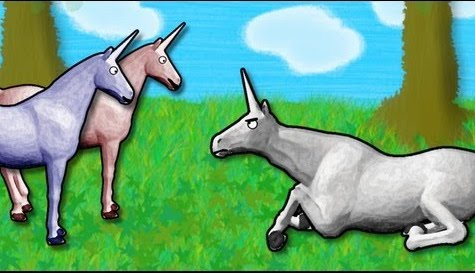
\includegraphics[scale=.5]{img/charlie}
	\ \\[.1in] 
	\caption*{ Charlie! We're going on an adventure, Charlie!}
	\label{fig:charlie}
\end{figure}

\frontrowcenter{Please note: This is a \makered{real} homework assignment, worth 20\% of your homework points.}

Watch the \href{https://www.youtube.com/watch?v=fZu3P0OsQPk}{entire saga} of {\em Charlie the Unicorn} on the YouTube channel \href{https://www.youtube.com/channel/UCV3iHQsE2h3CH-LehgPRkMg}{Filmcow} and answer the following questions. We will be referring to the other two annoying unicorns in the video(s) as \Redun{} and \Blueun, respectively.

% STUDENT: Replace all instances of \hrule or \hrulefill with \underline{your response}.

\begin{enumerate}[label=(\alph*)]
\setlength{\itemsep}{10pt}
 % \setlength{\parskip}{10pt}
  %\setlength{\parsep}{10pt}
	\setstretch{1.8}
	\item What is the name of the \textbf{location} that the unicorns are traveling to in their first adventure? \\  \hrule 
	\item According to Charlie, what did the \textbf{magical Liopleurodon} say? \hrulefill 
	\item What did the unicorns steal from Charlie at the end of the first adventure? \hrulefill
	\item What kind of \textbf{fish} are the two annoying unicorns ostensibly imagining in the beginning of the second adventure? \hrulefill 
	\item To whom must the unicorns return \textbf{the amulet}? \hrulefill 
	\item And, if they don't deliver the amulet, what will \textbf{the vortex} supposedly let out? \hrulefill \\ \hrule 
	\item What is the name of the \textbf{giant sneakertrain }that the unicorns must board to reach their second adventure destination? \hrulefill 
	\item According to the song sung by the creature in the end of the video, what must Charlie put \textbf{in his ear} in order to alleviate his general distress and everyday suffering? \hrulefill
		\item What did the unicorns steal from Charlie at the end of the second adventure? \hrulefill
		\item In the beginning of the third adventure, where do the annoying unicorns claim to be coming from? \\ \hrule
		\item What do \Redun{} and \Blueun{} want to employ Charlie's help with?\hrulefill
		\item Why do the unicorns need to be \textbf{silent}? \hrulefill
		\item Fill - in the following dialogue between Charlie,  \Redun{} and \Blueun{}.
					\begin{itemize}
							\em
							\item [-] \Blueun : Ring ring!
							\item[-] \Redun: Hello?			
							\item[-] \Blueun : Ring ring!
							\item[-] \Redun: He... he... hello?			
							\item[-] \Blueun : \hrulefill 
							\item[-] \Redun: \hrulefill 
							\item[-] \Blueun : \hrulefill 
							\item[-] \Redun: \hrulefill 
							\item[-] Charlie: \hrulefill 
					\end{itemize}							
			\item While underwater, what is \textbf{the first obstacle} that our unicorns have to pass in order to reach their final destination? \hrulefill 
			\item In the song that essentially culminates the third adventure, what kind of \textbf{sea creature} is \textbf{madly in love} with Charlie? \hrulefill
			\item What did the unicorns steal from Charlie at the end of the third adventure? \hrulefill
			\item What is the destination of the fourth and, as of the time of this writing, final adventure of our unicorns? \hrulefill 
			\item How did Charlie ``defeat" \textbf{the millepede}? \hrulefill 
			\item What did Charlie find inside the {\bf Cavern of the Red Wind}? \hrulefill
			\item What did \textbf{Starfish} say right at the end of the adventure? \hrulefill 
			\item {\em (1 pt extra credit)} In your opinion, what is the \textbf{meaning} behind Charlie the Unicorn, if any? \\[.1in] \Repeat{12}{\hrule \ \\} \hrule 
			
\end{enumerate}
\pagebreak

\problem{Syllabus / Deadlines}{18}

\frontrowcenter{To answer some of the questions of this problem, you will need to navigate our course's ELMS page and study our syllabus.}

% STUDENT: Replace all instances of \myline{...}  \underline{your response}.
\begin{enumerate}[label=(\alph*)]
\setlength{\itemsep}{1.5em}
	\item What is the due date of your \textbf{first} \textbf{homework}? \myline{2in}
	\item What is the date of your \textbf{first} midterm? \myline{2in}
	\item What is the date of your \textbf{second} midterm? \myline{2in}
	\item Where are \textbf{both} midterms taking place? \myline{2in}
	\item For what \textbf{percentage} of your \textbf{final score} do \textbf{all} of the \textbf{projects} count?  \myline{1in}
	\item For what \textbf{percentage} of your \textbf{final score} do \textbf{all} of the \textbf{midterm} {\bf and}  \textbf{final exams} \\ count? \myline{1in}
\end{enumerate} \vspace{-.2in}
 
 \pagebreak

\problem{Git basics}{22}

To pull the starter code for our projects, you will need to familiarize yourselves with the VCS \textbf{Git}, since the entire skeleton code will be hosted on a \href{https://github.com/JasonFil/CMSC420-Fall2018}{GitHub repository} that we maintain for you. To answer this problem effectively, you will need to study up on Git. Please navigate to the page named ``More Resources" on our \href{https://myelms.umd.edu/courses/1246980}{ELMS website} if you would like a starting point. Of course, Google is always your friend.

While a large subset of Git's functionality can be implemented using \href{https://git-scm.com/download/gui/linux}{various graphical tools}, there is {\bf no substitute} for the modularity, ease and cross-platform compatibility of using simple command line instructions from the shell. In this class, you will need to familiarize yourselves with a {\bf very basic} subset of available Git commands.

For every one of the following tasks, write the {\bf full} command that would be necessary to type on a command line in order for you to achieve the relevant task. Your answer should include: 
	\begin{itemize} \setlength{\itemsep}{.5em}
		\item The system program {\tt git}.
		\item The command to be passed to the program {\tt git} (e.g. {\tt add}, {\tt checkout}, {\tt push}, etc).
		\item Any flags to be passed to the command, e.g {\tt -b}, {\tt --cached}, {\tt -u}.
		\item Arguments that the command itself may need (e.g branch names, file paths, names of remotes, entire quoted strings, etc).
	\end{itemize}
	
You are {\bf quite encouraged} to try the commands out in your console before writing your responses below. In fact, the first four commands are a fine example of how you could start implementing your first project! We will provide you with the answer to the first question to help start you off. Note that this command does not have any \textbf{flags}, but it does, of course, have a URL argument.

% STUDENT: Replace all instances of  \item[] \gitproblemline with \item[] \underline{your response}. 
\begin{enumerate}[label=(\alph*)]
\setlength{\itemsep}{.8em}
	\item Clone the repository {\tt https://github.com/JasonFil/CMSC420-Fall2018.git} into the current directory, \textbf{using HTTPS}.
	\item[] \underline{\tt  \makered{git clone https://github.com/JasonFil/CMSC420-Fall2018.git } }
	\item Rename the remote {\tt origin} to {\tt classrepo}.
		\item[] \gitproblemline
	\item Rename the current branch to {\tt skeletoncode}.
		\item[] \gitproblemline
	\item Switch from the current branch to a {\bf new} branch called {\tt myimplem}.  
		\item[] \gitproblemline
	\item {\bf Stage} a Java source file which you just created and which you named {\tt MyStack.java}.
		\item[] \gitproblemline
	\item Make a \textbf{commit} from the current branch ({\tt myimplem}) with message ``Fixed stack popping issue.".
		\item[] \gitproblemline	\pagebreak
		\item Switch back to the branch {\tt skeletoncode}.
		\item[] \gitproblemline
		\item {\bf Merge} the branch {\tt myimplem} with the current branch, {\tt skeletoncode}.
	\item[] \gitproblemline
	\item \textbf{Push} your latest commit upstream.
		\item[] \gitproblemline
		\item List all your remotes.
			\item[] \gitproblemline
	\item Delete a remote called {\tt server2}.
		\item[] \gitproblemline
		\item Assuming you have applied changes to 10,000 different files (e.g by having your IDE automatically create \textbf{Scaladocs} for the entire code base of \textbf{Twitter}), type a \textbf{single command} that will stage  the files tracked by {\tt git} and to which the changes have been made.
		\item[] \gitproblemline
	\item Tweak your {\bf global, system-wide} Git configuration so that instead of typing {\tt git log -1 HEAD} to  \\ show your last commit's information, you could instead type the shorthand {\tt git last}.
		\item[] \gitproblemline
\end{enumerate}

\pagebreak

\problem{Sparse Matrix Representations}{20} 

Whether stored in column or row - major order, two-dimensional matrices can be a big bottleneck in terms of memory if they are \textbf{sparse}, that is, they have lots of {\tt null} cells. For example, the matrix shown in Table \ref{tbl:sparseMat} is quite sparse; only about $14\%$ of it is occupied!

\begin{table}[H]
    \centering
	\begin{tabular}{c | c c c c c c c c} 
		\  & \textbf{0} & \textbf{1} & \textbf{2} & \textbf{3} & \textbf{4} & \textbf{5} & \textbf{6} & \textbf{7} \\ \hline 
		\textbf{\Xt} & \textbf{11} & \Xt & \Xt & \Xt & \Xt & \Xt & \Xt & \Xt \\
		\textbf{1} & \Xt & \Xt & \Xt & \Xt & \Xt & $\mathbf{3}$ & \Xt & \Xt \\
		\textbf{2} & \Xt & \textbf{-3} & \textbf{4} & \Xt & \Xt & \Xt & \Xt & \Xt \\
		\textbf{3} & \Xt & \Xt & \Xt & \Xt & \Xt & \Xt & \Xt & \Xt \\	
		\textbf{4} & \Xt & \Xt & \textbf{11} & \textbf{6} & \Xt & \Xt & \Xt & $\mathbf{e^2}$ \\
		\textbf{5} & \textbf{-1} & \Xt & \Xt & \Xt & \Xt & \Xt & \Xt & \Xt \\
		\textbf{6} & \Xt & \Xt & \Xt & \Xt & \Xt & \Xt & $\mathbf{\sqrt{3}}$ & \Xt \\
		\textbf{7} & \Xt & \Xt & \Xt & \Xt & \Xt & \Xt & \Xt & \Xt \\	
	\end{tabular}
	\caption{A sparse matrix.  \Xt = \texttt{null} for brevity.}
	\label{tbl:sparseMat}
\end{table}

Programming languages such as {\tt MATLAB} offer built-in functionality (methods or operators included in the ``standard library" of the language) to {\em sparsify} a matrix. Sparsifying a matrix consists of transforming it into a l\textbf{inked list} which contains information {\em only for those cells of the matrix that have been filled in}. Every node of this list contains the $(i, j)$ coordinates of the relevant cell, as well as the data originally held in the cell. 

To answer some of the following questions, you will have to review {\bf asymptotic notation}. We have a resource page on ELMS (with CMSC250 slides linked) where you can review ``big-Oh" (\bigoh{$\cdot$}), ``big-Theta" (\bigtheta{$\cdot$}) and ``big-Omega" (\bigomega{$\cdot$}). 

For example, if you believe that a certain operation has time complexity {\em at most proportional to} $M$ (e.g, $2M, 2.5M, 4M - 7$), you should answer with \bigoh{$M$}. If instead you believe that it has time complexity at most proportional to the \textbf{square} of $M$ multipled by $N$ (e.g, $10 M ^2N + 2N$), you should answer with \bigoh{$M^2 N$}. If you believe that the operation runs in time {\bf exactly} proportional to $M^2 \cdot N$, you should answer with \bigtheta{$M^2 \cdot N$}.

\vspace{1in} 
\frontrowcenter{Questions on opposite page...}

\pagebreak

\begin{enumerate}[label=(\roman*)]
	\item Make a drawing of the sparsification of matrix shown in Table \ref{tbl:sparseMat}, assuming {\bf row-major} order. Recall what your nodes should contain.  \vspace{-.1in}
	
	% STUDENT: Replace \answerspace{}{}{} with your answer. Your drawing should be small enough 
	% FOR THE PAGE TO NOT BE DISRUPTED, i.e we want all questions, from (i) to (vi), to be in page 8.
	% We have to do this for Gradescope reasons. Look at the figure environment, the command 
	% \includegraphics and its parameter scale (e.g "\includegraphics[scale=.5]{img/myImg.png}).
	% Here's a full example of how to include an outside image in a nice centered format, with captions 
	%and all:
	
	%	\begin{figure}[H] % 'H' tells the LaTeX compiler that you want the figure exactly there in the 
									% doc,  not at the top of the page, not at the bottom, and certainly not in a 	
									% different or even the last page.
	%				\centering % Justifies your image centered
	%				\includegraphics[scale=.5]{path_to_my_img.png}
	%				\caption{My caption.}
	%				\label{fig:myLabel}
	%	\end{figure}
	% The purpose of \label{} is to allow you to refer to the Figure later in the document without 
	% having to remember which Figure is 1st, 2nd, or 24th. For example: "As we see in figure 
	% \ref{fig:myLabel} [...] "
	
	\answerspace{2in}
	
	\item Perform the same task, this time assuming {\bf column-major} order. \vspace{-.1in}
	
	% STUDENT: Same as above.

	\answerspace{2in}
	
	\item Suppose that our original matrix has dimensions $M \times N$. As a function of those two variables, and using \textbf{``big-Theta" (\bigtheta}{$\cdot$}\textbf{) notation}, what is the {\bf space} that the sparse matrix occupies in memory, in its \textbf{original} representation?  \myline{1in} 
	
	% STUDENT: In all those questions, simply replace \myline{} with \underline{your answer}. 
	\item Using the same notation, what is the space that the matrix occupies in its \textbf{sparsified} \\ format? \myline{1in}
	\item Suppose that $0 \leq i < M$ and $0 \leq j < N$. In its \textit{original} representation, what is the \textbf{time complexity} of assigning the cell ($(i, j)$) a value of, say, $3$ in the matrix's {\bf original} representation? \myline{1in}
	\item What is the time complexity of the same operation in the {\bf sparsified} representation? \myline{1in}
\end{enumerate}
\pagebreak

\problem{Memory representations of graphs}{20} 

Observe the graph of figure \ref{fig:graph}.

\begin{figure}[H]
	\centering
	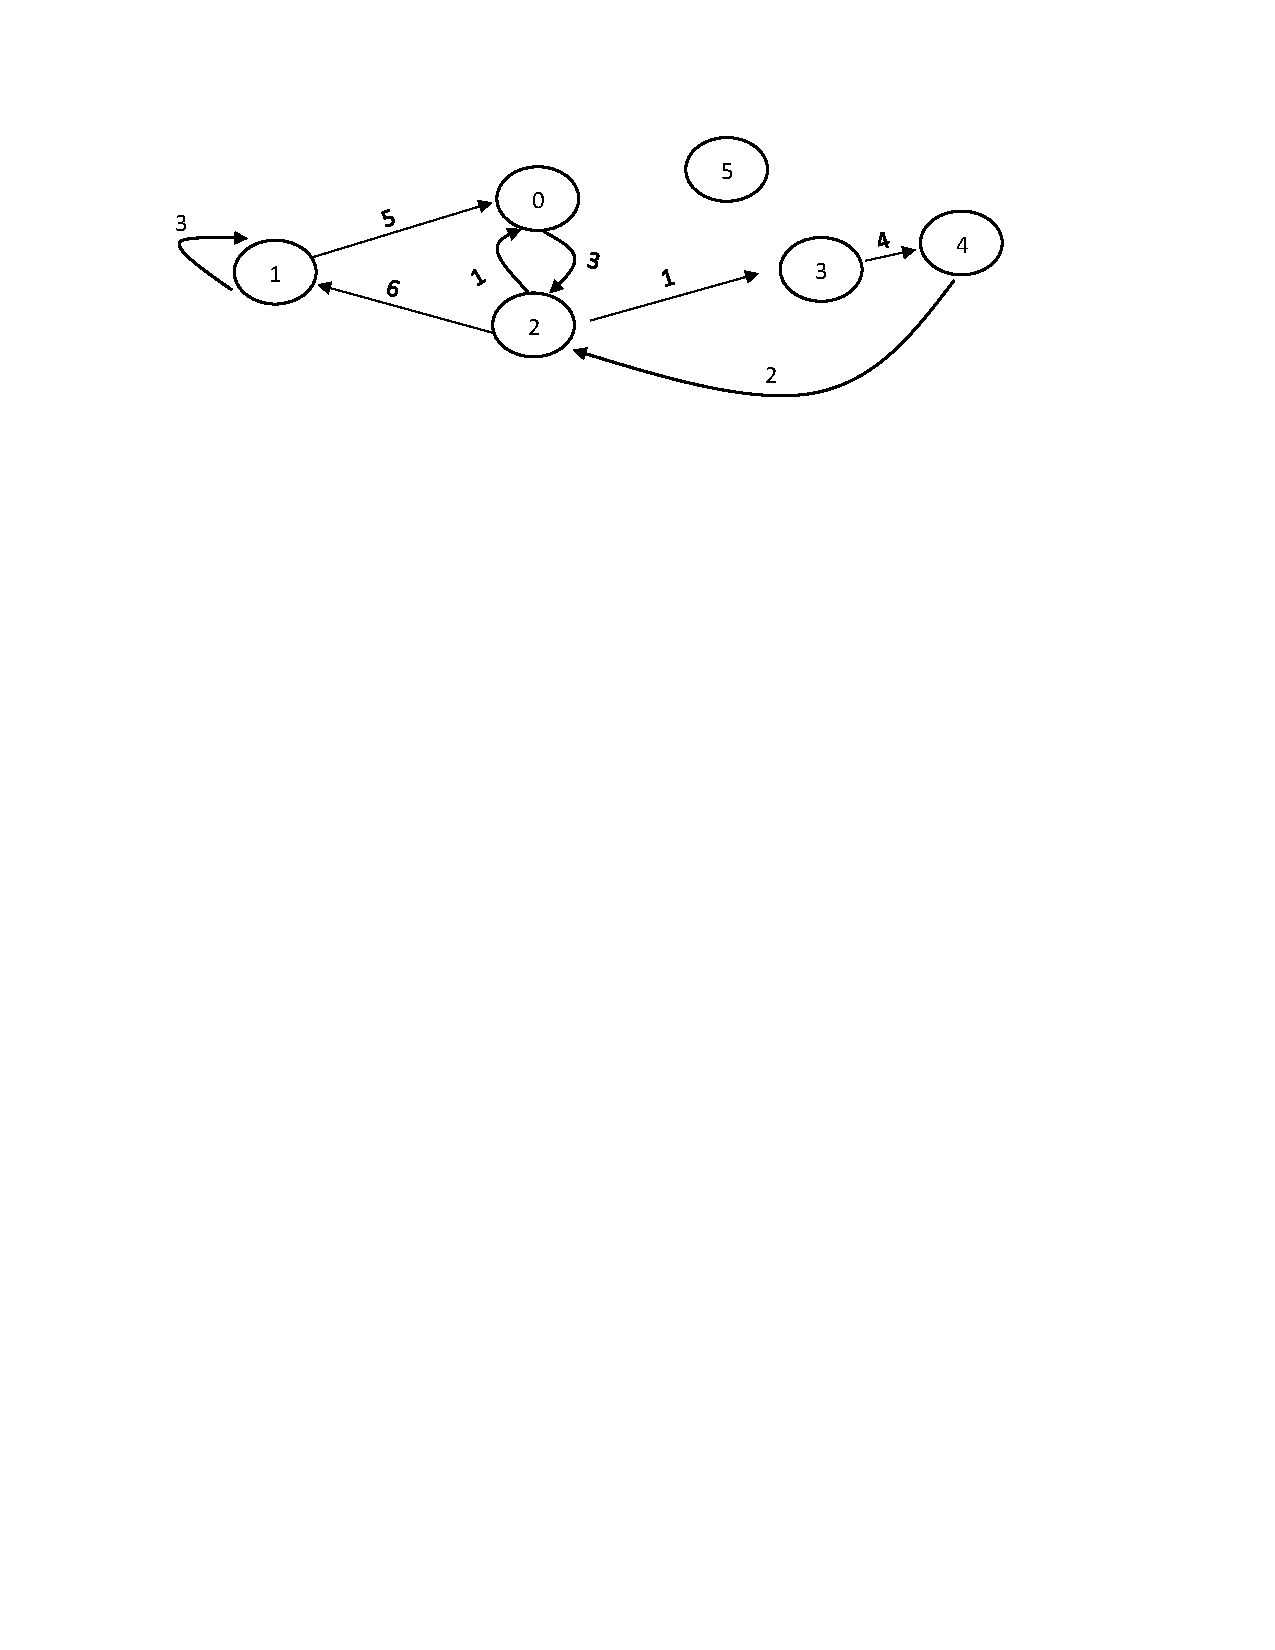
\includegraphics[scale=.9]{img/graph}
	\caption{A conceptual image of a graph. Nodes are enumerated from  $0$ (zero) \\ for consistency with later drawings.}
	\label{fig:graph}
\end{figure}

There are two common ways in which graphs, directed or undirected, are represented in computer memory: the {\bf adjacency matrix} (Table \ref{tbl:adjMat}) and the \textbf{adjacency list} (Figure \ref{fig:adjList}).  

\begin{table}[H]
	\centering
		\renewcommand*{\arraystretch}{1.5}
	\begin{tabular}{|c|c|c|c|c|c|c|} \hline
			&   \textbf{0} & \textbf{1} & \textbf{2} & \textbf{3} & \textbf{4} & \textbf{5} \\ \hline
		\textbf{0} & 0  & 0 & 3 & 0 & 0  & 0 \\ \hline
		\textbf{1} & 5  & 3 & 0 & 0 & 0 & 0 \\ \hline
		\textbf{2} & 1  & 6 & 0 & 1 & 0 & 0 \\ \hline
		\textbf{3} & 0  & 0 & 0 & 0 & 4 & 0 \\ \hline
		\textbf{4} & 0 & 0 & 2 & 0 & 0 & 0 \\ \hline 
		\textbf{5} & 0 & 0 & 0 & 0 & 0 & 0 \\ \hline 
	\end{tabular} 
	\caption{The {\bf adjacency matrix} representation of the graph of Figure \ref{fig:graph}.}
	\label{tbl:adjMat}
\end{table}

Let $V$ be the number of {\bf nodes} (or vertices) in a given graph $G$ and $E$ be the number of its \textbf{edges}. The adjacency matrix is a $V \times V$ matrix $M$ where: 

$$M(i, j) = \begin{cases} w, & \textit{where } w > 0 \textit{ is the weight of the edge } i \rightarrow j \\ 0,  & \textit{if there is no edge } i \rightarrow j \end{cases}$$

In \textbf{unweighted} graphs, $w = 1$ for all edges. 

{\bf Undirected} graphs, on the other hand, have the interesting property that their adjacency matrix is   {\bf symmetric}: 

$$(\forall i , j \in \{ 1, 2, \dots , V \})[M(i, j ) = M(j, i)]$$. 

The {\bf adjacency list} representation of this graph is a single-dimensional array $A$ of length $V$, defined as follows:

$$A(i) = \{ v,\ \textit{if vertex } v \textit{ is connected to vertex  } i \textit{ in } G \}$$

\begin{figure}[H]
		\centering
		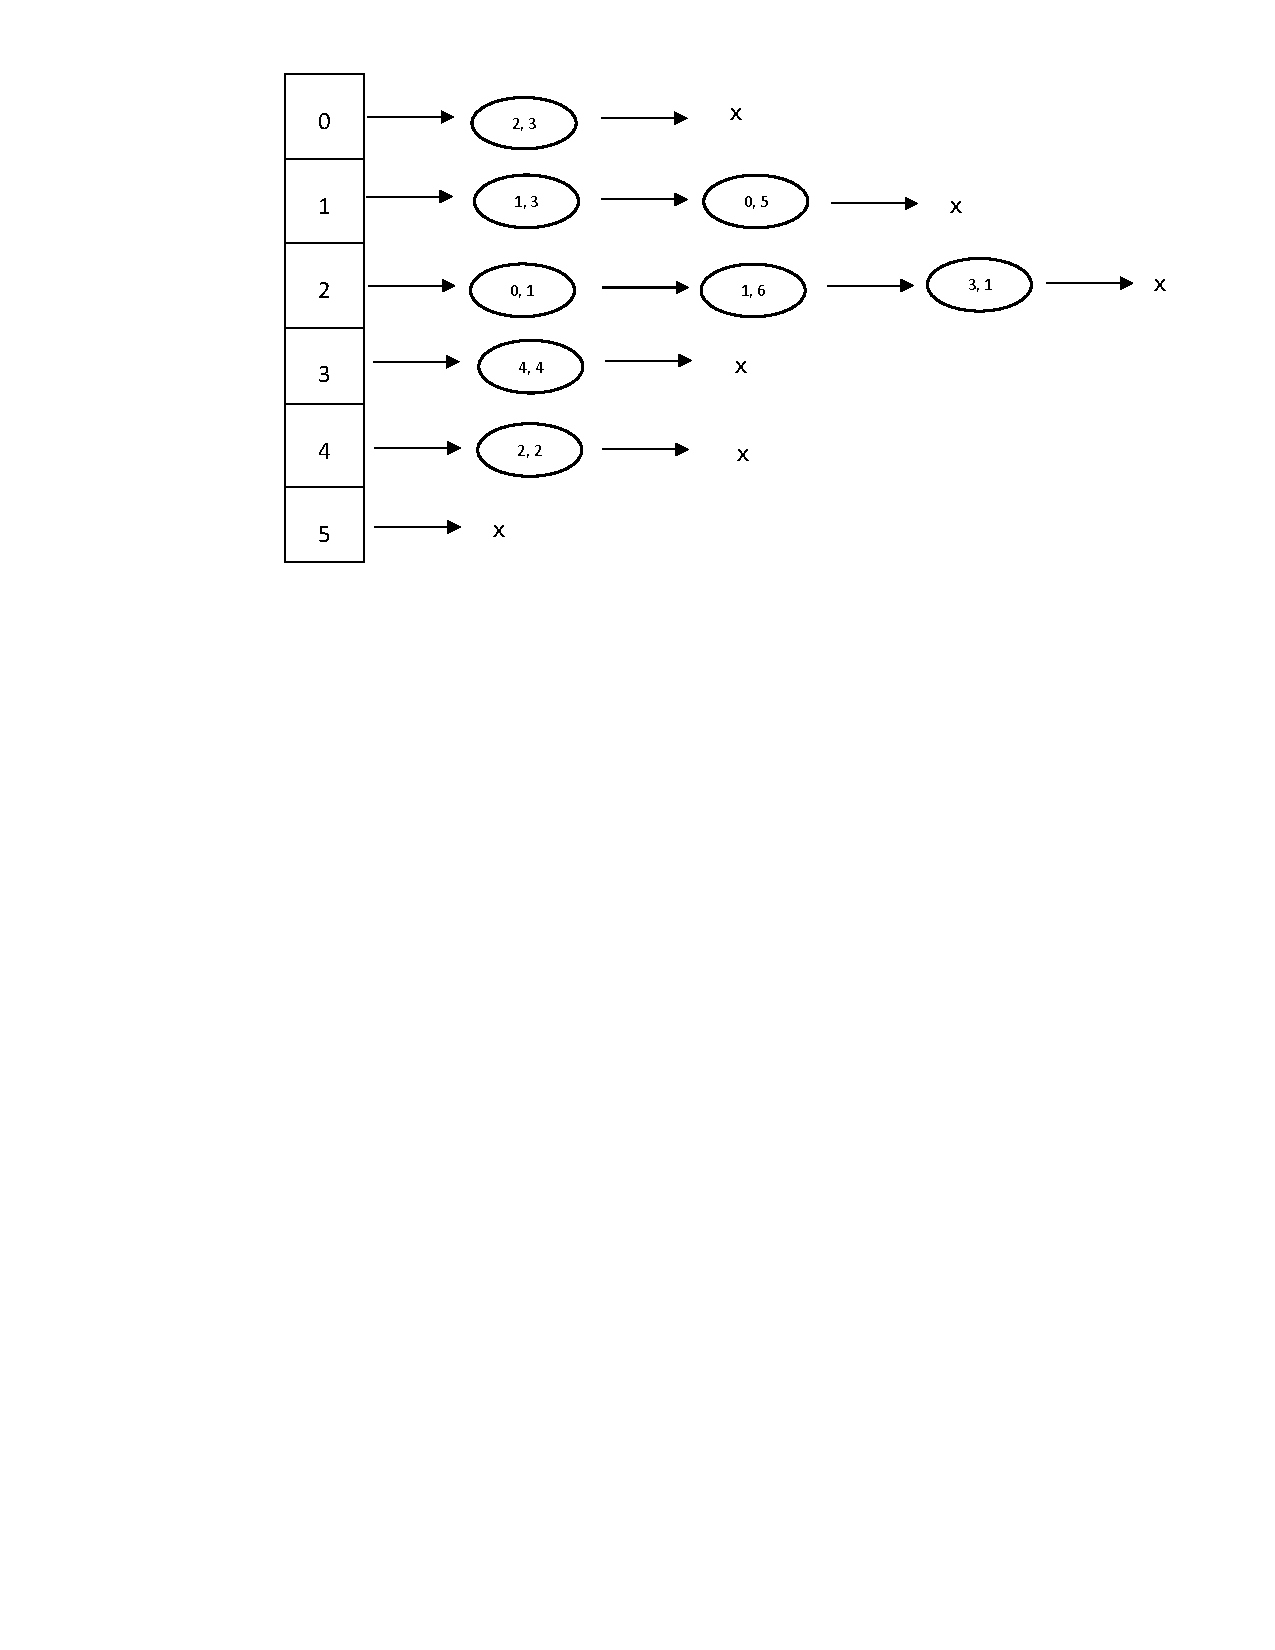
\includegraphics[scale=.8]{img/adjList}
	\caption{The {\bf adjacency list} representation of the graph of Figure \ref{fig:graph}. Every node \\ in the list contains a tuple (\textbf{target\_node\_id, weight}).}
	\label{fig:adjList}
\end{figure}

So $A(i)$ points to the \textbf{set} of all vertices $v$ on which $i$ is incident. These sets are typically organized as \textbf{linked lists}, as implied by Figure \ref{fig:adjList}. These lists do \textbf{not have to be sorted in any way}. For this question, we will assume that:

	\begin{itemize}
		\item The heads of the sets are contained in a classic, one-dimensional contiguous storage array ({\bf not} a ``dynamic" array like Java's {\tt ArrayList} and C++'s {\tt Vector}). So the entire adjacency list representation will consist of an \textbf{array of lists} (see Figure \ref{fig:adjList}).
		\item The lists themselves are organized as {\bf classic, bare-bones linked lists}. This means that we will {\bf not} endow these lists with a pointer to their last element, and we will also {\bf not} have a link pointing to the previous node from every node (i.e the linked lists are {\bf not} doubly-connected) (see Figure \ref{fig:adjList}).
	\end{itemize} 
	
Furthermore, we add a little twist to these representations, based on information from problem 4. We will consider a {\bf sparse adjacency matrix} representation of this graph (linked list of only non-{\tt null} elements). Figure \ref{fig:sparseAdjMat} shows how the graph of Figure \ref{fig:graph} is represented in such a format.

\begin{figure}[H]
		\centering
		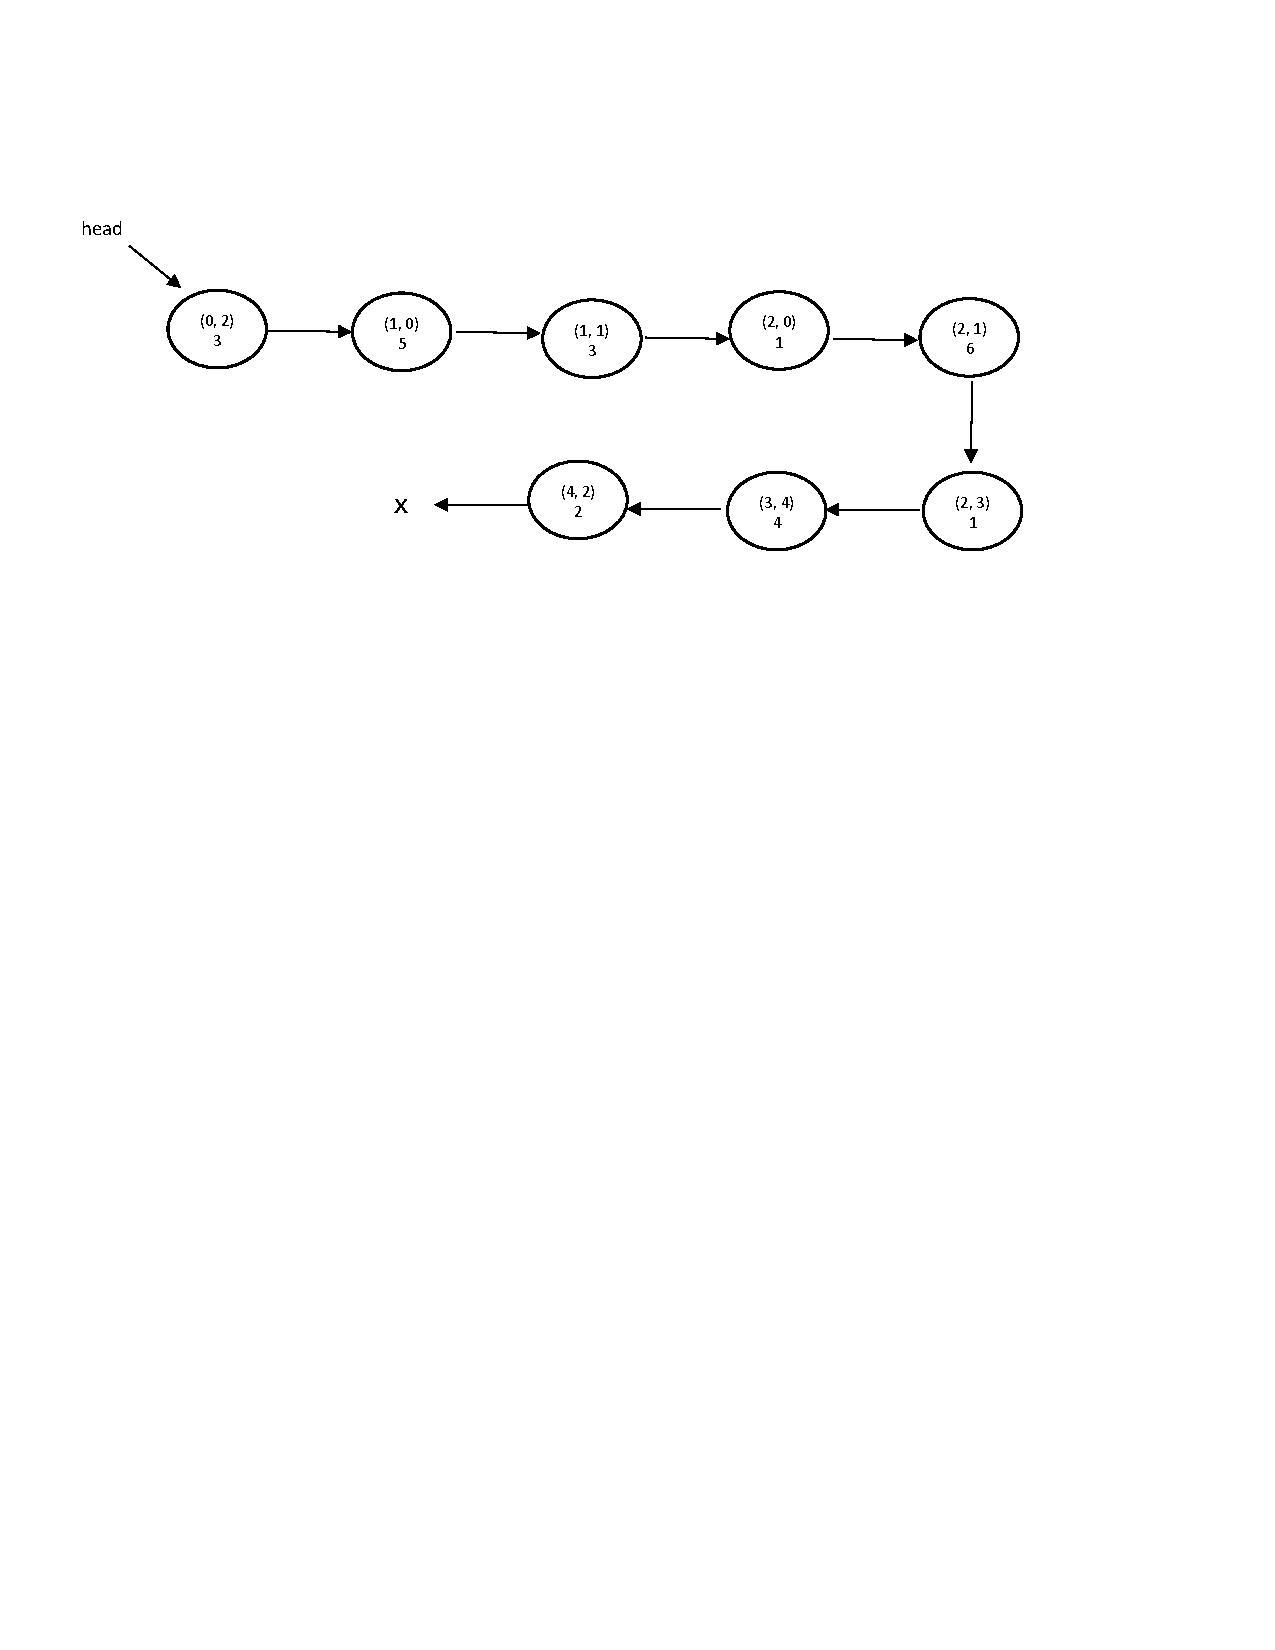
\includegraphics[scale=.8]{img/sparseAdjMat}
		\caption{The {\bf sparse adjacency matrix} representation of the graph of Figure 
		\ref{fig:graph}. The matrix has been scanned in row-major order (but does it really matter which order we use?)}
	\label{fig:sparseAdjMat}
\end{figure}

 Your task is to fill-in Table \ref{tbl:complexities} using appropriate complexity notation, coupled with the parameters $V$ and $E$. For example, if you believe that a certain operation will take time \textit{proportional} to the {\bf cube} of the number of nodes $V$, you should answer with \bigoh{$V^3$}. Or, if you believe that the operation will take time proportional to the product of vertices multiplied by the logarithm base 2 of the number of edges $E$, you should answer \bigoh{$V \cdot \log_2E$}. Finally, also consider the fact that $0 \leq E \leq V^2$, since the ``worst case" for the number of edges in a graph is $V^2$, for a $V$-clique.

% STUDENT: You have to place your answer in between the appropriate ampersands ('&') below.
% For example, if you want to fill-in the top-leftmost cell, you would need to write down your answer % in between the 1st and 2nd ampersand of the first line of the table.

\begin{table}[H]
	\centering
	\renewcommand*{\arraystretch}{2.0}
	\begin{tabular}{|p{4.5cm}|c|c|c|} \hline
		\textbf{Operation} & \textbf{Adjacency Matrix} & \textbf{Adjacency List} & \textbf{Sparse Adjacency Matrix} \\ \hline
		Is node $i$ \textbf{connected} to node $j$? & & & \\ \hline
		Add a new \textbf{node} $k$. & & & \\ \hline
		Add the \textbf{edge} $i \rightarrow j$. & & & \\  \hline
		Remove a \textbf{node} $\ell$. & & & \\ \hline
		Remove the \textbf{edge} $i \rightarrow j$.  & & & \\ \hline
		Spatial Complexity & & & \\  \hline
	\end{tabular}
	\caption{Fill in this table with appropriate asymptotic notation.}
	\label{tbl:complexities}
\end{table}		

\vspace{.8in}

\end{document}